In this chapter, we first discuss the evaluation metrics typically used for
classification problems. In Section~\ref{sec:feat_extraction} we explore classic
and novel forms of feature extraction and feature combinations for audio
problems. Section~\ref{sec:classification} categorises popular models used for
audio classification problems, both old and new.

\section{Evaluation metrics}\label{sec:eval_metrics}

For multiclass classification problems, e.g.\ identifying a sample as a
particular bird species from a list of $n > 2$ species, a simple classification
accuracy is often used as an evaluation
metric~\cite{chakraborty2016bird,ramashini2022robust}. This is calculated as
the percentage of correctly identified samples from a set of labelled samples
previously unseen by the model. A high accuracy indicates a performant model.

Acevedo et al.~\cite{acevedo2009automated} used true positive rate (TPR) and false
positive rate (FPR) to evaluate their models used to classify bird and amphibian
calls, defined as
\begin{equation}
  \text{TPR} = \frac{\text{TP}}{\text{P}}, \hspace{1em}
  \text{FPR} = \frac{\text{FP}}{\text{N}}
\end{equation}
where TP and FP are the numbers of true positives and false positives
respectively, and P and N are the number of real positive and real negative
classes in the data. This evaluation method is sometimes preferred when
analysing long recordings which may include several different species to be
classified. TPR indicates how well the model correctly identifies
species present in the recording. FPR indicates how often the model erroneously
identifies species absent in the recording. A high-performing model will have
high values for TPR and low values for FPR\@.

Potamitis et al,~\cite{potamitis2014automatic} used an alternative form of
evaluation presented in terms of precision $(P)$ and recall $(R)$ which are
defined as
\begin{equation}
  P = \frac{\text{TP}}{\text{TP}+\text{FP}}, \hspace{1em}
  R = \frac{\text{TP}}{\text{TP}+\text{FN}}
\end{equation}
where FN is the number of false negatives. Informally, $P$ and $R$ can be
thought of as
\begin{equation}
  P = \frac{\text{relevant retrieved instances}}{\text{all \textbf{retrieved} instances}}, \hspace{1em}
  R = \frac{\text{relevant retrieved instances}}{\text{all \textbf{relevant} instances}}
\end{equation}

$P$ and $R$ are unhelpful metrics when reported in isolation. For example, it's
possible to achieve perfect recall in a multiclass birdsong classification
problem by simply assigning a sample to all possible classes. Note that in this
example the precision will be close to 0\@. It's therefore desirable to achieve
a high precision and a high recall, however, it's well known that there is a
trade-off between $P$ and $R$. Improving one metric often leads to a decrease in
the other metric. Due to this, the $F$-score is often reported along with the
$P$ and $R$ metrics. The $F$-score is defined as
\begin{equation}
F = \frac{(1+\beta^2)PR}{\beta^2P + R}
\end{equation}
for some $\beta \in \mathbb{R}$. The $\beta$ is chosen such that recall is
considered $\beta$ times as important as precision. Usually, the $F_1$ score is
presented, where $\beta = 1$.

For binary classification problems, i.e.\ classifying a sample as one of two
classes (bird species), the Area Under Curve (AUC) metric is sometimes
preferred~\cite{leng2014multi}. It is calculated as the area under a receiver
operating characteristic (ROC) curve, which plots TPR vs FPR at different
classification thresholds, see Figure~\ref{fig:roc} for an example. The AUC
ranges from 0 to 1, with a higher value indicating a better-performing model.
The AUC is sometimes desirable because it is scale-invariant (it measures how
well predictions are ranked, rather than their absolute values) and
classification-threshold-invariant (it measures the quality of the model's
predictions regardless of what classification threshold is chosen.)

\begin{figure}[ht]
  \centering
  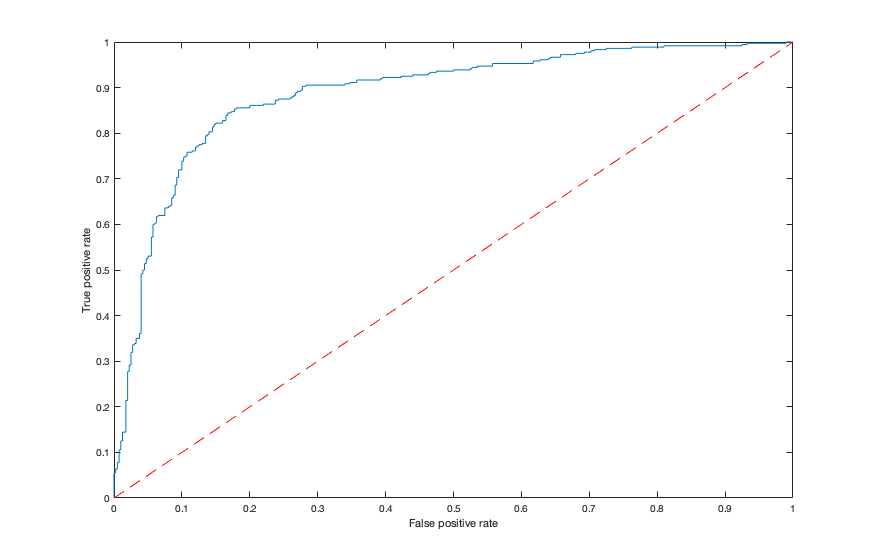
\includegraphics[width=\textwidth]{figures/roc.png}
  \caption{Example ROC curve for a reasonably performant model, shown in blue.
  The red dashed line indicates the baseline for binary classification problems:
a model outputting random predictions. The AUC is calculated as the area under
the blue curve.}\label{fig:roc}
\end{figure}

\section{Feature extraction}\label{sec:feat_extraction}

As mentioned in Chapter~\ref{cp:intro}, birds use vocalisations as a way to
communicate with others. Birds have evolved over many thousands of years to make
this form of communication very efficient in that it can travel long distances
and cut through local ambient noise so that it can be received by other birds
clearly. Some birds have even adapted their vocalisations so that they can be
heard in local environments that have rapidly changed over the past decades,
such as urban areas with increasing anthropogenic noise~\cite{luther2010urban}.

Bird vocalisations can be broadly divided into two main categories, calls and
songs. Calls are typically short vocalisations that carry some specific
function, such as warning others of the presence of a predator or calling others
to flight~\cite{MARLER2004132}. Songs are usually longer, more acoustically
complex, and occur more spontaneously. They are typically employed as breeding
calls or territorial defence. While all birds produce calls, in many species of
birds only the males utilise songs and often only during the breeding season. The
song and call of a Eurasian wren can be seen and contrasted in
Figure~\ref{fig:wren_call_song_spectrogram}.

\begin{figure}[ht]
  \centering
  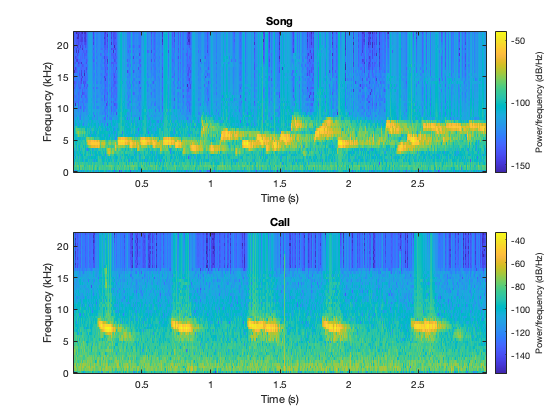
\includegraphics[width=\textwidth]{figures/wren_call_song_spectrogram.png}
  \caption{Spectrograms of a call and song of a Eurasian wren
  (\textit{Troglodytes troglodytes}). As can be seen, the song is much more
complex in terms of pitch and acoustic structure compared to the
call.}\label{fig:wren_call_song_spectrogram}
\end{figure}

Doupe et al.~\cite{birdsongspeech} showed that there were striking similarities
between birdsong and human language. Similar to human language, birdsong can be
thought of as consisting of hierarchical levels of phrases, syllables, and
elements~\cite{catchpole2003bird}. The levels for a common chaffinch can be seen
in Figure~\ref{fig:syllables}. Raw recordings of birdsong
often contain periods of silence that occur between phrases which are unlikely
to provide useful information to train a machine learning model.
Fagerlund~\cite{fagerlund2007bird} showed that a good level of accuracy can be
achieved by training models on features extracted from segmented syllables which
were used as training samples. An algorithm for robust syllable segmentation was
proposed in~\cite{fagerlund2004automatic} and is used in this thesis. The
algorithm is described in more detail in Section~\ref{ssec:syllable_seg}.

\begin{figure}[ht]
  \centering
  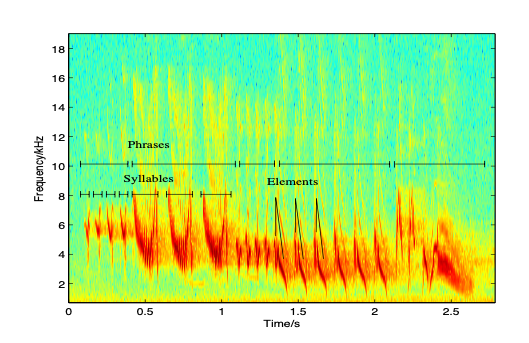
\includegraphics[width=0.8\textwidth]{figures/syllables.png}
  \caption{Spectrogram showing the hierarchical levels of the song of a common
  chaffinch. Figure taken from~\cite{fagerlund2004automatic}.}\label{fig:syllables}
\end{figure}

Once the syllables have been segmented, there exists an abundance of options to
turn the raw syllable input signal into features that might be used as training
samples. In the following sections, some of the more popular feature
representations are described, along with some novel methods that have yet to be
tried on birdsong. Note that the following list is certainly not exhaustive and
emphasis has been placed on feature representations that are relevant to this
thesis.

\subsection{Features inspired by the human auditory system}

Research has shown that birdsong and human language share many similarities in
terms of the neural mechanisms employed to form the language/song and the impact
of social contact in learning the language/song~\cite{birdsongspeech}. Given that
the human auditory system has evolved over thousands of years to best process
human speech, it seems reasonable to suggest that using features based on the
human auditory system may be effective when it comes to birdsong.

At a high level, the human auditory system works by translating changes in air
pressure originating from a source and reaching the outer ear of a listener
into vibrations that travel along an internal organ known as a cochlea. The
vibrations trigger electric signals that move along auditory nerves to the
brain, where they are interpreted as sounds. The physiology of the cochlea
means that specific parts of it are more sensitive to specific frequencies
of vibrations, so different frequencies will lead to different electrical
signals moving to the brain. This allows the brain to learn to differentiate
between frequencies.

\subsubsection{Mel frequency cepstrum coefficients}

The makeup of the human auditory system means that humans have a greater ability
to differentiate pitch at lower frequencies than they do at higher frequencies.
In other words, humans perceive pitch non-linearly. This has led to the
development of a logarithmic frequency scale, known as the mel scale, such that
equal distances on the scale have the same \textit{perceptual} distance.

The mel frequency cepstrum coefficients (MFCC) are part of a family of cepstrum
coefficients that capture information about the rate of change in different
spectrum bands. MFCC differs from other cepstrum coefficients in that it uses the
mel scale to transform the spectrum of an input signal, thus utilising the human
auditory system in the calculation of its coefficients. This is done by passing
a signal through a bank of filters that are spaced according to the mel scale.

The $i$-th mel cepstral coefficient is computed as~\cite{davis1980comparison}
\begin{equation}
\text{MFCC}_i = \sum_{k=1}^{K} X_k \cos \left(
  \frac{i(k-0.5)\pi}{K}
\right)
\end{equation}
where $X_k$ is the logarithmic energy of the $k$-th mel-spectrum band, and $K$
is the total number of the mel-spectrum bands. Usually 8--13 MFCC coefficients
are used as the feature vector representing one time frame of the signal. The
0$^{th}$ coefficient is often excluded as it represents the average log energy
of the signal and is unlikely to carry any relevant information to help with
classification.

MFCCs are often presented with their delta ($\Delta$) and double-delta
($\Delta\Delta$) values that capture the local temporal dynamics and temporal
changes of the delta values respectively.

MFCCs are used as feature representations since they are simple to compute and
have been shown to have good performance in a wide range of audio classification
tasks, such as speaker identification~\cite{muda2010voice} and emotion
recognition~\cite{likitha2017speech}. MFCCs have also been shown to lead to good
classification accuracy for birdsong identification
problems~\cite{fagerlund2007bird,ramashini2022robust}.

\subsubsection{Gammatone cepstrum coefficients}

Gammatone cepstrum coefficients (GTCCs) are similar to MFCCs except their
calculation  uses gammatone filterbanks instead of mel scale filterbanks.
Gammatone filterbanks are designed to simulate the motion of the membrane inside
the cochlea, known as the basilar membrane, when it is exposed to vibrations
transmitted by the outer and middle ear~\cite{patterson1992complex}.

A gammatone filter with a centre frequency $f_c$ is defined as
\begin{equation}
  g(t) = at^{n-1}e^{-2\pi b t} \cos(2\pi f_c + \psi)
\end{equation}
where $t$ is the time in seconds, $\psi$ is the phase in radians (usually set to
0), $a \in \mathbb{R}$ controls the gain, $n$ is the filter's order and $b$ is
the filter's bandwidth in Hz. To simulate the human auditory system, the centre
frequencies are uniformly spaced on the equivalent rectangular band-width (ERB)
scale.

Similar to MFCCs, GTCCs are typically used with their $\Delta$ and $\Delta\Delta$
values and have also been shown to have a good performance in
non-speech audio classification problems~\cite{valero2012gammatone}.

For the Eurasian wren song shown in Figure~\ref{fig:wren_call_song_spectrogram},
the MFCC and GTCC coefficients can be seen in
Figure~\ref{fig:mfcc_gtcc_example}. Note that this visualisation does not
include the $\Delta$ and $\Delta\Delta$ values and also includes the
$0^{\text{th}}$ coefficient, denoted as $\log E$ in the figure.

\begin{figure}[ht]
  \centering
  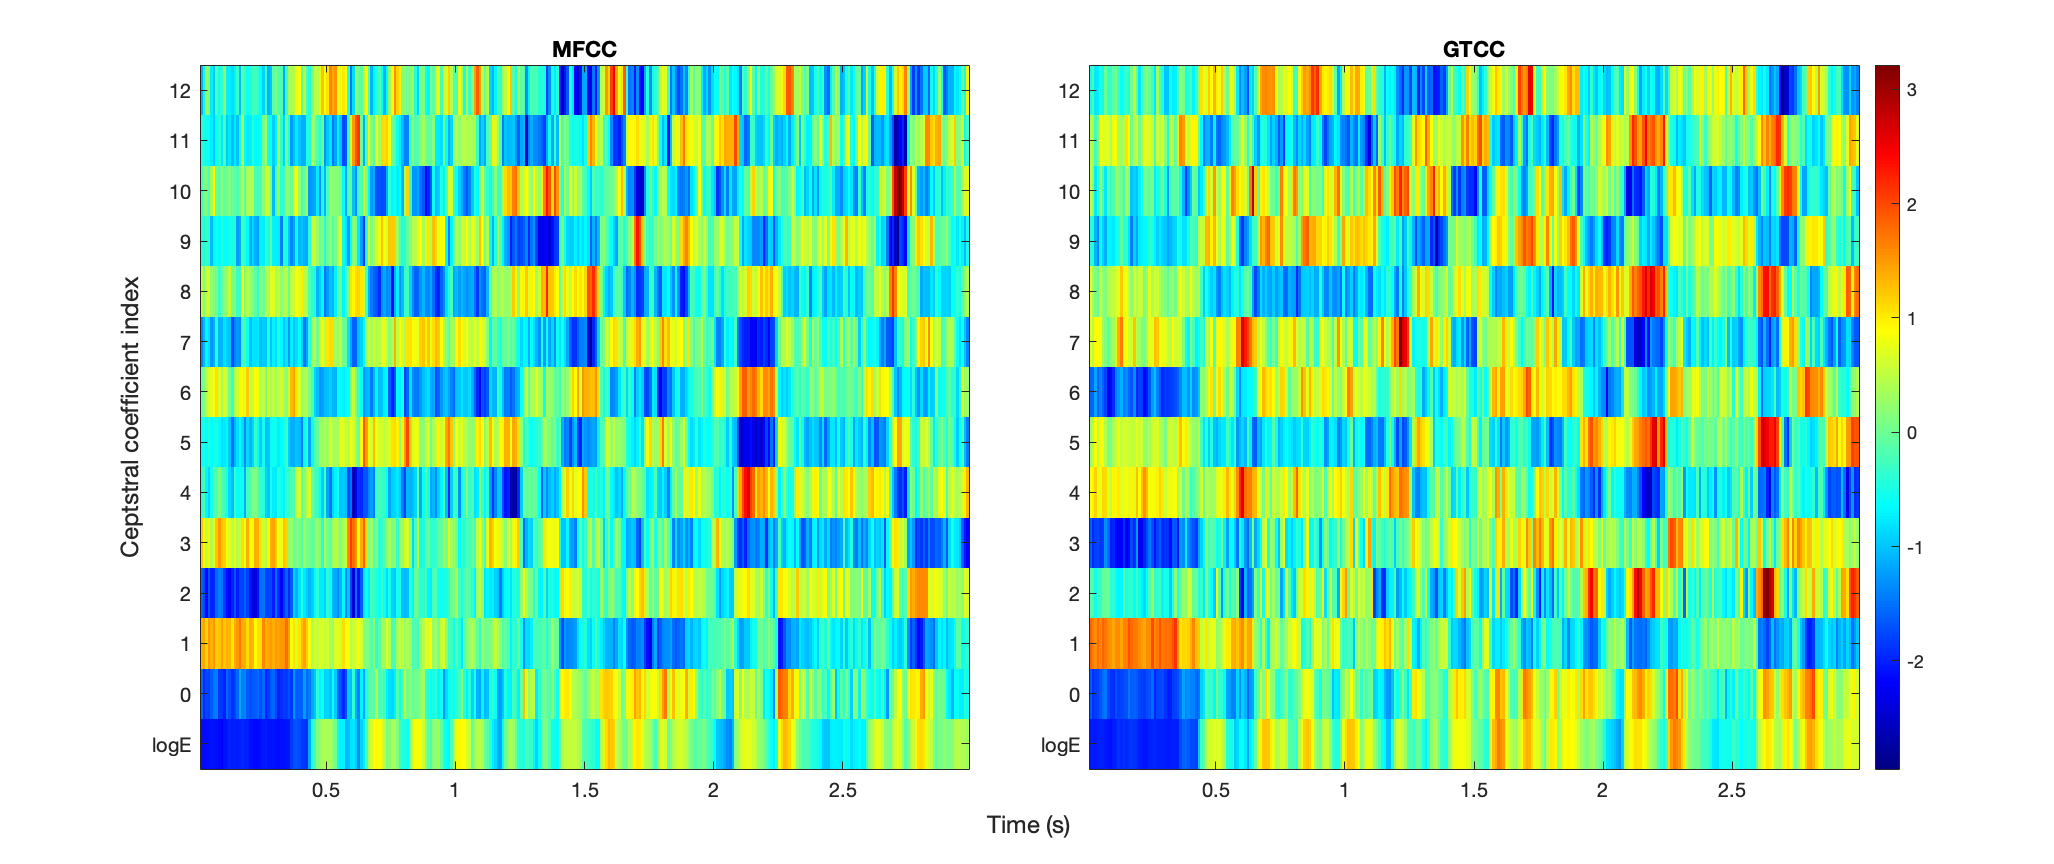
\includegraphics[width=\textwidth]{figures/mfcc_gtcc_example.png}
  \caption{MFCC and GTCC coefficients for a sample of Eurasian wren
  birdsong.}\label{fig:mfcc_gtcc_example}
\end{figure}

\subsubsection{Multi resolution cochleagram}

Chen et al.~\cite{chen2014feature} proposed a novel feature known as a
multi-resolution cochleagram (MRCG) that is formed by combining four
cochleagrams at different resolutions, designed to capture both local and
contextual information.

A cochleagram is formed by passing an input signal through a gammatone
filterbank, similar to the first steps of the formation of the GTCCs\@. Each
response signal from the gammatone filterbank is then divided into frames of a
certain length with a certain overlap or frame shift. The cochleagram is then
generated by calculating the power of each frame at each channel.

A MRCG is formed by first taking one cochleagram with a frame length of 20ms and
frame shift of 10ms, using a gammatone filterbank with 64 output channels. A log
operation is applied to each time-frequency (T-F) unit of the output
cochleagram, denoted CG1. CG2 is calculated in the same way, but with a frame
length of 200ms and the same frame shift. CG3 is calculated by averaging CG1
across a square window of 11 frequency channels and 11 time frames centred at
the given T-F unit. Zero padding is used here. CG4 is calculated in the same way
as CG3, but with a $23 \times 23$ square window. CG1--4 are then stacked
vertically to obtain the full MRCG feature, which will be a $256 \times p$
matrix, where $p$ is the number of time frames. The MRCG for the Eurasian wren
song shown in Figure~\ref{fig:wren_call_song_spectrogram} can be seen in
Figure~\ref{fig:mrcg_example}.

\begin{figure}[ht]
  \centering
  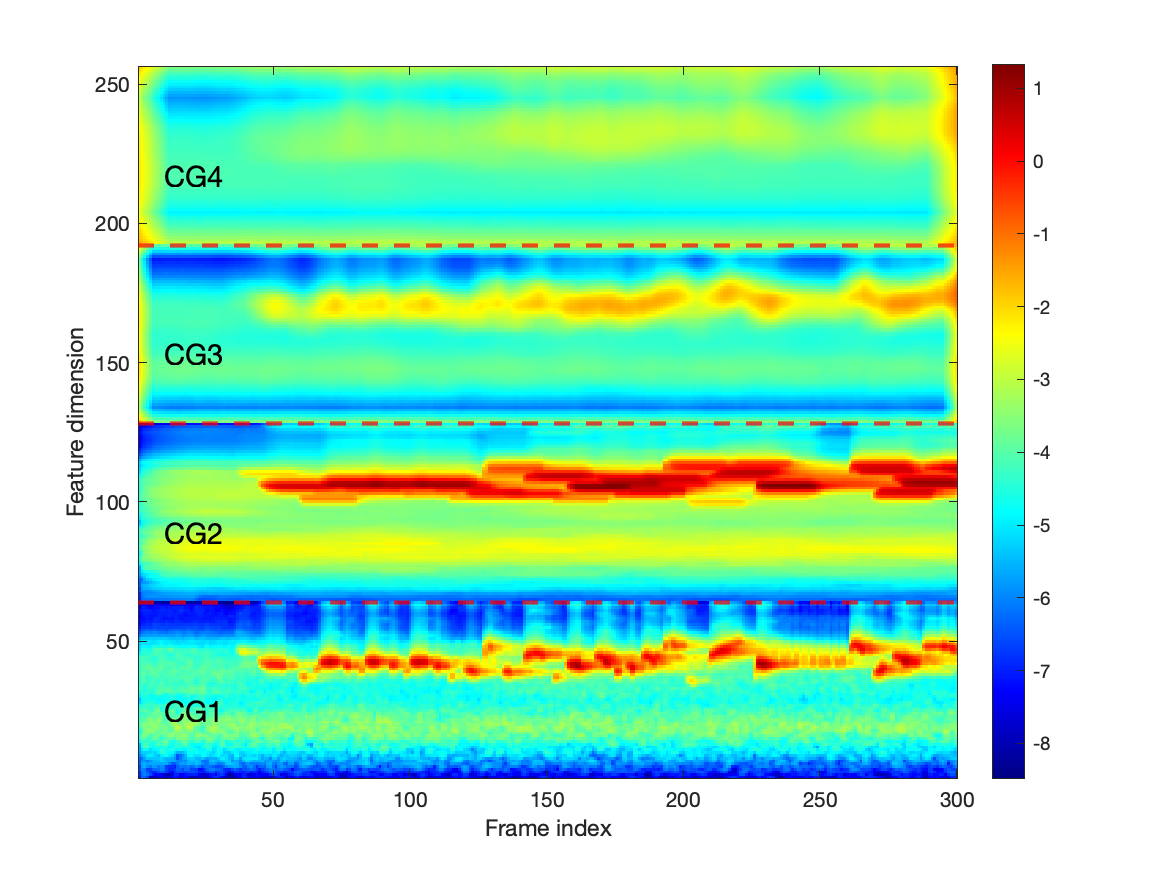
\includegraphics[width=0.9\textwidth]{figures/mrcg_example.png}
  \caption{MRCG of sample of Eurasian Wren birdsong. The component cochleagrams
  are labelled CG1--4 and the red dashed lines indicate the boundaries
between cochleagrams.}\label{fig:mrcg_example}
\end{figure}

The MRCG feature has been shown to outperform both MFCC and GTCC at
separating human speech at various SNR levels with different types of
background noise~\cite{chen2014feature}. Abdullah et
al.~\cite{binti2020comparison} showed that the MRCG outperforms the Auditory
Image Model (AIM) when classifying noise. Wang et al.~\cite{wang2016joint} showed
that improved speech enhancement for hearing impaired listeners was achieved
when the MRCG feature was added to the feature set.

One potential drawback when comparing the MRCG with MFCC and GTCC is the higher
dimensionality of the MRCG feature. When including the $\Delta$ and
$\Delta\Delta$ features, as is standard
practice~\cite{binti2020comparison,wang2016joint}, the MRCG feature vector for a
single time frame has a dimensionality of 768. For MFCC or GTCC the equivalent
dimensionality is 24--39, depending on the number of the coefficients used.

\subsection{Feature stacking}

It has been shown that an appropriate combination of features to be used as
training inputs can lead to improved classification accuracy in audio related
problems such as speech separation~\cite{wang2012exploring}. Ramashini et
al.~\cite{ramashini2022robust} showed that a combination of GTCC and MFCC yielded
higher birdsong classification accuracy than MFCC alone. However, the
combination did not improve on the accuracy of GTCC alone. Yan et
al.~\cite{yan2021birdsong} demonstrated that a combination of MFCC with two other
feature types (Log-mel spectrogram and Chroma) yielded higher birdsong
classification accuracy than combinations of two of the features alone.
Fagerlund~\cite{fagerlund2007bird} showed that combining MFCC with spectral and
temporal features, such as frequency range and zero crossing rate, can lead to
higher birdsong classification accuracies.

A consequence of feature stacking is that feature vectors will have increased
size. This can lead to problems such as longer training times and overfitting,
especially when used in conjunction with deep learning (DL) architectures. As a
result, dimensionality reduction techniques such as Principal Component
Analysis (PCA) or Linear Discriminant Analysis (LDA)~\cite{ramashini2019bird}
are often used to reduce the dimensionality of the feature vectors while still
capturing enough information to be able to train a model effectively.

\section{Classification}\label{sec:classification}

Once a suitable feature representation has been selected and extracted, the
remaining task is to pick an appropriate model and train the model using the set
of training samples generated from the feature extraction.

There exist many different options in terms of models, and no one model is
superior to the others. Each problem must be considered and a model which fits
the problem at hand must be selected, or indeed a selection of suitable models
tested and then evaluated for performance.

In the literature, birdsong classification has been tackled with a wide variety
of models. Ramashini et al.~\cite{ramashini2019bird} used the simple Nearest
Centroid (NC) classifier to assign birdsong samples to classes. It was compared
to a K Nearest Neighbours (KNN) classifier and shown to have superior accuracy.
Lasseck~\cite{lasseck2015improved} used decision trees with bagging to identify
birds. Trifa et al.~\cite{trifa2008automated} used Hidden Markov Models (HMM) to
identify species of birds based on their vocalisations. They considered each
sample as a discrete-time dynamical system, where an unobserved state generates
observed features, such as pitch and MFCC\@. A different HMM can be learned for
each class and a new sample can be assigned to a class by calculating which HMM
gives the highest likelihood of the observed features. Kwan et
al.~\cite{kwan2006automated} used a Gaussian Mixture Model (GMM) to classify
birds. In their experiments, a Gaussian was learned for each class of bird. A
new sample was then classified according to whichever class best describes the
new sample.

The following sections describe some models that are relevant to this thesis in
more detail

\subsection{SVMs}

SVMs are widely used in machine learning applications as a classification tool.
They are well-established due to their high accuracy
results~\cite{fagerlund2007bird} and relative simplicity to implement. Many
implementations of SVMs also require little or no tuning of hyperparameters.

At its core, a SVM is a binary classifier that separates two classes by finding
a hyperplane that maximises the margin from the nearest vectors in the feature
space from both classes. Classifications are then made by computing on which
side of the hyperplane a test feature vector lies.

\subsubsection{Binary classification}

Let $\mathbf{x}_i \in \mathbb{R}^m$ be a feature vector of dimensionality $m$.
Let $y_i \in \left\{ +1, -1 \right\}$ be its class label. For linearly separable
data, the separating hyperplane satisfies
\begin{equation}\label{eq:svm_hyperplane}
y_i\left( \left< \mathbf{w} \cdot \mathbf{x}_i \right> + b \right) \ge 1, \hspace{1em}
i = 1,\ldots,n
\end{equation}
where $\mathbf{w} \in \mathbb{R}^m$ is a vector of weights and $b \in
\mathbb{R}$ is a bias term. The margin between the hyperplane and the nearest
feature vectors from each class is given by
\begin{align}
  \text{d}(\mathbf{w},b) &=
  \min_{\mathbf{x}_i,y_i=1}
  \frac{|\left< \mathbf{w} \cdot \mathbf{x}_i \right> + b|}{\|\mathbf{w}\|} +
  \min_{\mathbf{x}_j,y_i=-1}
  \frac{|\left< \mathbf{w} \cdot \mathbf{x}_j \right> + b|}{\|\mathbf{w}\|} \\[0.5em]
                         &= \frac{2}{\|\mathbf{w}\|}. \label{eq:svm_margin}
\end{align}

The optimal hyperplane can now be found by maximising (\ref{eq:svm_margin})
subject to (\ref{eq:svm_hyperplane}). This can be solved using Lagrange
multipliers.

Often with real world data, classes are not linearly separable. This can
be remedied by projecting the data using a nonlinear mapping into a new feature
space where the data are linearly separable. Equation (\ref{eq:svm_hyperplane})
can then be rewritten as
\begin{equation}\label{eq:svm_nonlinear_mapping}
y_i\left( \left< \mathbf{w} \cdot \boldsymbol{\Phi}(\mathbf{x}_i) \right> + b \right) \ge 1, \hspace{1em}
i = 1,\ldots,n
\end{equation}
where $\boldsymbol{\Phi}$ is the nonlinear mapping. Instead of explicitly
finding $\boldsymbol{\Phi}$, (\ref{eq:svm_nonlinear_mapping}) can be re-written
in dual form
\begin{equation}
y_i\left(
  \sum_{j=1}^{l} \alpha_j y_j \left<
  \boldsymbol{\Phi}(\mathbf{x}_j) \cdot \boldsymbol{\Phi}(\mathbf{x}_i)
  \right>
\right) + b \ge 1, \hspace{1em} i=1,\ldots,n
\end{equation}
and replacing the inner product with a kernel function
$K(\mathbf{x}_j,\mathbf{x}_i) = \left< \boldsymbol{\Phi}(\mathbf{x}_j) \cdot
\boldsymbol{\Phi}(\mathbf{x}_i) \right>$.

In practice, a hyperplane that separates the classes perfectly may suffer from
poor generalisation ability. To improve this, nonnegative slack variables
$\xi_i$ are introduced to (\ref{eq:svm_nonlinear_mapping}) to allow for some
missclassification of training samples to improve generalisation
ability. The slack variables are introduced like so
\begin{equation}\label{eq:svm_nonlinear_mapping_slack}
y_i\left( \left< \mathbf{w} \cdot \boldsymbol{\Phi}(\mathbf{x}_i) \right> + b
\right) \ge 1 - \xi_i, \hspace{1em}
i = 1,\ldots,n
\end{equation}
The amount of regularization is controlled by the constant $C$ such that the
maximisation problem (\ref{eq:svm_margin}) becomes
\begin{equation}
\frac{2}{\|\mathbf{w}\|} - C \sum_{i=1}^{n} \xi_i
\end{equation}

Therefore for large values of $C$ the classifier will behave like a hard-margin
SVM and attempt to perfectly classify all training samples.

The last remaining question is around what determines a valid kernel function. A
function in the input space is a kernel function if its kernel matrix
$\mathbf{K} = \left[ K(\mathbf{x}_j,\mathbf{x}_i) \right]^{n}_{i,j=1}$ is
positive semidefinite. Typical kernel functions include
\begin{itemize}

  \item linear: $K(\mathbf{x}_j,\mathbf{x}_i) = \left< \mathbf{x}_j, \mathbf{x}_i \right>$

  \item polynomial: $\left(\left< \mathbf{x}_j, \mathbf{x}_i \right> + c\right)^p$
    for some $c \in \mathbb{R}$

  \item Gaussian or RBF\@: $\exp \left( -\gamma \|\mathbf{x}_j-\mathbf{x}_i\|^2 \right)$
    for some $\gamma \in \mathbb{R}, \gamma > 0$.

\end{itemize}

\subsubsection{Multiclass classification}\label{sssec:multiclass}

SVMs can easily be extended to work with multiclass classification using
standard procedures. One such procedure which is optimal with respect to the
Hamming Loss, which relates to the number of false positives or false negatives,
is the one-versus-all technique. Here, multiple SVMs are trained, each one
learning the hyperplane for samples belonging to one class versus samples
belonging to all the other classes. A new sample can then be tested against all
the models and predictions are made using the model that is most confident.

\subsection{Neural Networks}\label{ssec:nn}

Although neural networks (NN) have existed in some form since the 1950s with the
inception of the perceptron algorithm~\cite{rosenblatt1958perceptron}, they have
experienced a huge surge in popularity over the past decade or so. This has
largely been due to remarkable progress being made thanks to deep neural
networks in fields such as image classification~\cite{krizhevsky2012imagenet}
and language models~\cite{mikolov2010recurrent}.

Another reason for DL's increasing popularity in recent years is due to the
availability of more performant hardware and software. The `deep' aspect to deep
learning refers to the fact that the software architecture depends on large
amounts of parameters and needs massive amounts of training data to learn. In
order to run training routines in a reasonable time and store large amounts of
data in memory, access to powerful hardware and/or machine parallelism tools can
be an essential part of the process.

The progress of audio related problems has also been accelerated due to deep
neural networks. Hinton et al.~\cite{hinton2012deep} showed improved performance
in speech recognition tasks using feed-forward neural networks when compared to
more classical approaches like HMMs and GMMs. Speech
enhancement~\cite{afouras2018conversation} and speech
separation~\cite{ephrat2018looking} problems leveraging DL paradigms
have also been shown to outperform more classical statistical models.

The world of birdsong classification has also benefited from DL, but perhaps to
a lesser extent than other audio related problems so far. Approaches have mainly
focused on Convolutional Neural Networks (CNNs), applying convolutional layers
to an image representation of an input signal, such as a
(Mel-)spectrogram~\cite{berger2018bird,mukherjee2018convolutional}. Further
birdsong classification solutions have approached the problem in a similar
fashion, but utilised transfer learning to fine-tune an existing
model~\cite{disabato2021birdsong,lasseck2018acoustic}, such as
ResNet~\cite{he2016deep} and ImageNet~\cite{deng2009imagenet}.

Disabato et al.~\cite{disabato2021birdsong} went a step further with their
research in that they considered the computational and memory demands of their
proposed bird detection DL network, ToucaNet. As mentioned earlier, DL
applications can be extremely demanding in terms of computational resources
which can make them unsuitable for running on devices with limited resources,
such as smartphones and autonomous recording units (ARUs). Their research showed
that a level of accuracy in line with the literature can be achieved but with
lower computational complexity and memory demands.

Although the architecture of DL tools for birdsong classification may vary
widely, the final layer is typically the same. This consists of a fully
connected layer of $n$ units, where $n$ is the number of classes, with a softmax
activation so that the output of the network can be considered as a probability
distribution over the classes. The softmax function is defined as
\begin{equation}
\sigma{(\mathbf{z})}_i = \frac{e^{z_i}}
  {\sum_{j=1}^{K} e^{z_j}}, \hspace{1em} i = 1,\ldots,K
\end{equation}
where $K$ is the number of classes.

A classification of an unseen sample can then be performed by assigning the
sample to the class with the highest corresponding probability.

\subsubsection{Feedforward Neural Network}

A feedforward neural network (FNN) consists of a system of connected nodes,
organised in layers, where information flows in one direction only --- forward
--- from the input nodes, through the hidden nodes (if any), and to the output
nodes. This differs fundamentally from e.g.\ a RNN, where information can flow
forward and backward. However, both FNNs and its derivatives and RNNs share
many similarities, such as learning using backpropagation, and using nonlinear
activation functions to model nonlinear data.

A FNN in perhaps its most basic form while still being able to solve non-trivial
problems is known as a multilayer perceptron (MLP). An MLP consists of at least
three layers of fully connected nodes with a nonlinear activation function, see
Figure~\ref{fig:mlp}. Since their inception in late 21$^{\text{st}}$ century
MLPs have had extensive research conducted into their capabilities and
efficiency~\cite{hornik1989multilayer}.

\begin{figure}[ht]
  \centering
  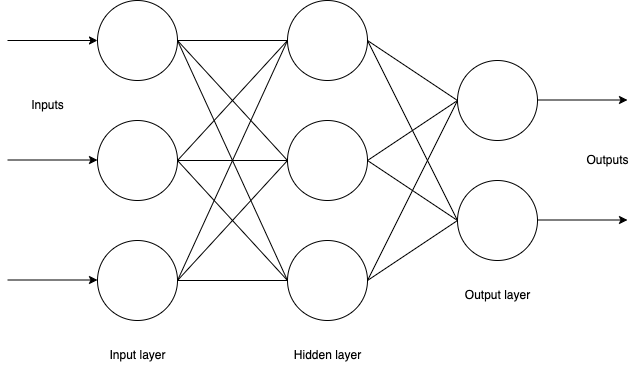
\includegraphics[width=0.8\textwidth]{figures/mlp.png}
  \caption{An example of a simple MLP\@. Data flows into the network from the
  input layer, through the hidden layer, and out the output layer.}\label{fig:mlp}
\end{figure}

MLPs have largely been superseded by more modern DL architectures such as CNN and
RNN when it comes to audio problems such as birdsong classification, however
there have been examples of more vanilla neural networks being used. McIlraith
and Card~\cite{mcilraith1997birdsong} used a two layer perceptron network using
backpropagation to minimize a mean squared error loss to classify samples from 7
birds. Murcia and Paniagua~\cite{murcia2013bird} used a simple FNN to classify
birdsong from 35 different bird species, achieving 0.74 AUC and in doing so
winning the International Conference on Machine Learning Bird Challenge 2013.

\subsubsection{Convolutional Neural Network}

CNNs have seen a big surge in development and popularity over the last decade,
largely thanks to huge strides being made in fields like machine vision and
image classification using architectures such as
AlexNet~\cite{krizhevsky2012imagenet}. Since image and audio share many
conceptual similarities, it is reasonable to suggest that CNNs may enjoy similar
success in the world of audio classification problems. This hypothesis is
strengthened when one considers that many feature representations of audio
signals can be displayed as images, such as spectrograms
(Figure~\ref{fig:wren_call_song_spectrogram}), MRCG outputs
(Figure~\ref{fig:mrcg_example}) and MFCC outputs
(Figure~\ref{fig:mfcc_gtcc_example}). Indeed, there has been significant
progress in recent years thanks to CNNs in fields such as audio event
recognition~\cite{takahashi2017aenet} and automatic speech
recognition~\cite{sercu2016very}.

A CNN is a feedforward neural network with at least one convolutional layer. A
convolutional layer is so called because it performs a convolution on an input,
usually an image, using a small matrix of weights, known as a filter or kernel.
The output is considered as a matrix of activations. The activation is higher
when the values in the corresponding area of the input are similar to those in
the kernel, meaning that the activation output encodes the location of where the
input matches certain features. Usually, several kernels are applied at each
layer, and so the output takes the shape of a 3D matrix, or a volume. As with
all neural nets, the output is passed through a nonlinear activation function in
order to allow for the network to be able to learn from nonlinear data. The
weights in the kernel are learned through backpropagation. Usually a max
pooling layer is added to downsample the activation volume and reduce
the number of weights, or parameters, needed by the network. An example of a
simple CNN can be seen in Figure~\ref{fig:cnn_example}.

\begin{figure}[ht]
  \centering
  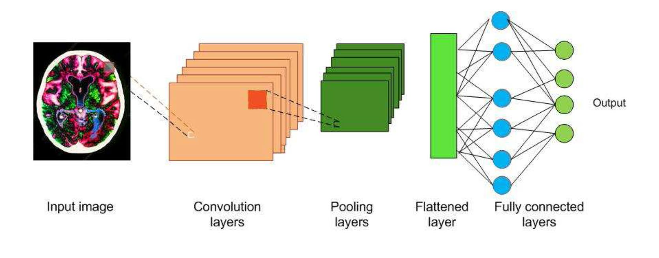
\includegraphics[width=\textwidth]{figures/cnn_example.png}
  \caption{An example of a simple CNN architecture. This network operates on
  images of brain scans and outputs a class from one of 4 options. Figure taken
from~\cite{sarvamangala2022convolutional}.}\label{fig:cnn_example}
\end{figure}

CNNs lend themselves well to image related problems since their structure allows
them to parse an image as a composition of meaningful elements rather than a
collection of unrelated pixels~\cite{lecun2015deep}. This translates well to
birdsong as e.g.\ a spectrogram of a sample of birdsong can conceptually be
thought of as a composition of syllables, i.e.\ elements.

CNNs have been applied to birdsong classification challenges with great success.
Kahl et al.~\cite{kahl2017large} achieved a remarkable mean average precision of
0.605 for a dataset of 1500 different bird species using a CNN trained on
spectrograms of 4 second samples. The spectrograms were pre-processed to reduce
noise and augmented with a variety of augmentations, such as adding Gaussian
noise and real noise samples from the original dataset. Ruff et
al.~\cite{ruff2020automated} used CNNs to detect owl vocalisations in
spectrograms from unprocessed field recordings, performing as well or better
than human experts. Narasimhan et al.~\cite{narasimhan2017simultaneous} used a
CNN with encoder-decoder architecture based on
Segnet~\cite{badrinarayanan2017segnet} to simultaneously segment and classify
birdsong spectrograms. This approach benefits from the fact that segmentation
and classification are intuitively strongly correlated, since when comparing
two different segmentations, the one that leads to a higher classification
accuracy will likely be a better segmentation.

\subsubsection{Recurrent Neural Network}

Since FNNs have a fixed size of input and output, they become unsuitable when
either the input size is variable and the output is fixed (e.g.\ with AI image
generation tools like Dall-E~\cite{ramesh2021zero}), the input size is fixed and
the output is variable (e.g.\ image captioning) or both the input size and
output size are variable (e.g.\ language translation). RNNs solve this problem
by allowing information in the network to flow in directed cycles. This is done
by feeding the output from a previous step as input to the current step, meaning
that the state of the hidden units depends on the previous state of the network.
This gives the network the ability to learn long term dependencies thanks to an
unbounded previous history. The architecture of a vanilla RNN cell is shown in
Figure~\ref{fig:rnn_cell_example}.

\begin{figure}[ht]
  \centering
  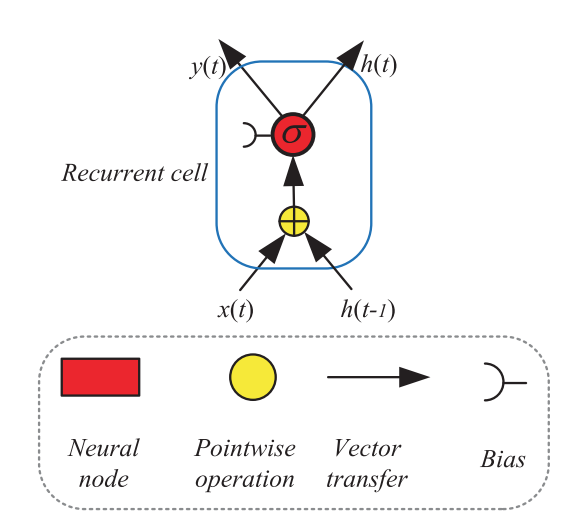
\includegraphics[width=0.6\textwidth]{figures/rnn_cell_example.png}
  \caption{Diagram of a vanilla RNN cell. Here, the input $x(t)$ at time $t$ is
    combined with the hidden state at the previous timestep $h(t-1)$
    and fed into the neural node. The output takes the form of a traditional
    activation $y(t)$ and a new hidden state $h(t)$ to be used with the
    next input $x(t+1)$. Figure taken
  from~\cite{yu2019review}.}\label{fig:rnn_cell_example}
\end{figure}

Similar to FNNs, classification RNNs learn by minimizing a loss function,
usually the cross-entropy loss~\cite{shore1980axiomatic}, by backpropagation.
However, a slight variation on the algorithm is used to incorporate the
sequential nature of the input data. The variation is known as backpropagation
through time (BPTT). Here, to update the weights matrices, all weights
are first treated as independent. The standard backpropagation algorithm is then
run and all the corresponding gradients are averaged together. BPTT however
suffers from a problem whereby gradients larger than 1 are multiplied together,
which causes the gradient updates further back the network to exponentially
increase, which may cause numerical instability and memory problems during
training. This is known as the gradient exploding problem. The equivalent
problem whereby gradients less than 1 vanish towards 0 is known as the gradient
vanishing problem. This results in the model having no ability to learn long
term dependencies. Both of these problems are compounded by RNNs learning from
long sequences of inputs, causing longer multiplicative chains of updates. The
gradient exploding problem can be tackled using strategies such as gradient
clipping, whereby the gradient is reset to a small number after it exceeds a
threshold value using 
\begin{equation} 
  g = \frac{\text{threshold}}{\|g\|}g
\end{equation}

A common approach to dealing with the gradient vanishing problems is to replace
vanilla RNN cells with long short-term memory (LSTM) units or gated recurrent
units (GRU).

\subsubsection{LSTM}

LSTM was first proposed by Hochreiter and Schmidhuber~\cite{hochreiter1997long}
and has seen excellent results in fields such as speech
recognition~\cite{he2016exploiting} and acoustic
modelling~\cite{qu2017syllable}. LSTM describes an alternative structure for RNN
whereby the hidden units are replaced with a memory cell which can store
information for extended periods. The flow of information in and out of
the cell is controlled by three boolean gates: a forget gate (\ref{eq:lstm_f})
which controls how information is lost from memory, an
input gate (\ref{eq:lstm_i}) which controls how new information is stored in
memory, and an output gate (\ref{eq:lstm_o}) which controls which information in
memory should be output to the next layer and for the next time step.
\begin{align}
  f(t) &= \sigma(W_f \cdot \left[ h(t-1),x(t) \right] + b_f) \label{eq:lstm_f} \\[0.5em]
  i(t) &= \sigma(W_i \cdot \left[ h(t-1),x(t) \right] + b_i) \label{eq:lstm_i} \\[0.5em]
  o(t) &= \sigma(W_o \cdot \left[ h(t-1),x(t) \right] + b_o) \label{eq:lstm_o} \\[0.5em]
  \tilde{c}(t) &= \tanh \left( 
    W_c \cdot \left[ h_{t-1},x_t \right] + b_{\tilde{c}}
  \right)\\[0.5em]
  c(t) &= f(t) \odot c(t-1) + i_t \odot \tilde{c}(t) \\[0.5em]
  h(t) &= o(t) \odot \tanh (c(t))
\end{align}

Here, $\odot$ represents the Hadamard product (element-wise multiplication) and
$W_{\{f,i,o,c\}}$ and $b_{\{f,i,o,c\}}$ are trained weights matrices and biases
respectively. The above equations describe how an input vector $x(t)$ at time
step $t$, the previous hidden state $h(t-1)$ and cell state $c(t-1)$ combine to
compute the next hidden state $h(t)$ and cell state $c(t)$. This process can be
visualised in Figure~\ref{fig:lstm_cell_example}.

\begin{figure}[ht]
  \centering
  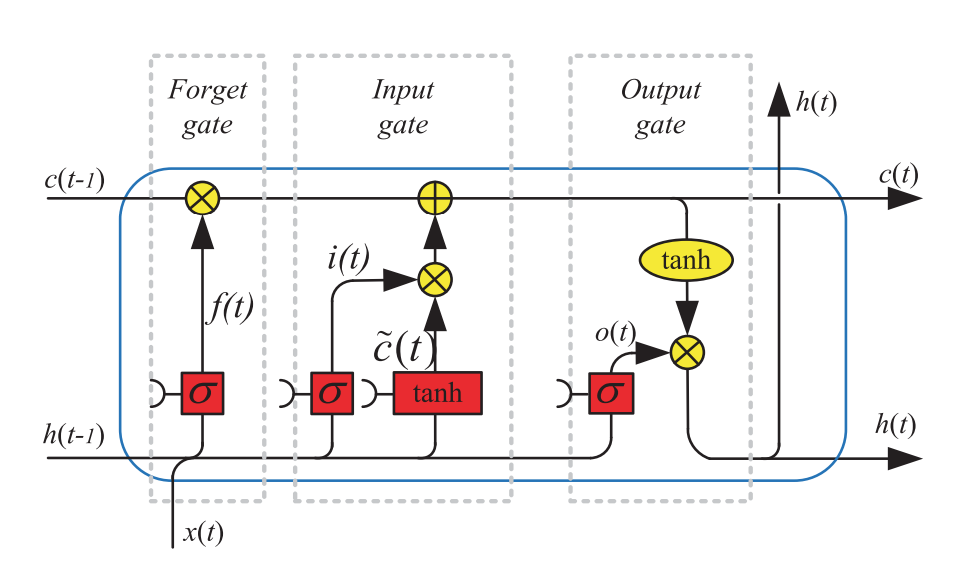
\includegraphics[width=0.8\textwidth]{figures/lstm_cell.png}
  \caption{Diagram showing the structure of a LSTM cell. As with the vanilla RNN
    cell shown in Figure~\ref{fig:rnn_cell_example}, the $x(t)$ and $h(t-1)$
    combine but this time with a cell state $c(t-1)$. The output now takes the
    form of a new cell state $c(t)$ and hidden state $h(t)$. Figure taken
  from~\cite{yu2019review}.}\label{fig:lstm_cell_example}
\end{figure}

The key conceptual difference between LSTM and RNN is that LSTM separates memory
from the hidden state. LSTM deals with the gradient vanishing problem since the
memory cells are additive with respect to time~\cite{daniluk2004automatic}. 

\subsubsection{GRU}

GRU was first proposed by Cho et al.~\cite{cho2014properties}. GRU shares many
similarities with LSTM in that it replaces hidden units in a RNN with a memory
cell, however it improves on LSTM in that it has fewer parameters, and therefore
has lower computational burden. The reduction in parameters is achieved by
combining the input gate and the forget gate of an LSTM to form an update gate,
meaning that the GRU has only two gates, an update gate (\ref{eq:gru_z}) and a
reset gate (\ref{eq:gru_r}). The GRU cell can be seen in
Figure~\ref{fig:gru_cell}.

\begin{align}
  r_t &= \sigma\left( W_{rh}h_{t-1} + W_{rx}x_t + b_r \right) \label{eq:gru_r} \\[0.5em]
  z_t &= \sigma\left( W_{zh}h_{t-1} + W_{zx}x_t + b_z \right) \label{eq:gru_z} \\[0.5em]
  \tilde{h}_t &= \tanh\left( W_{hh}(r_t \odot h_{t-1}) + W_{hx}x_t + b_z \right) \\[0.5em]
  h_t &= (1-z_t) \odot h_{t-1} + z_t \odot \tilde{h}_t
\end{align}

\begin{figure}[ht]
  \centering
  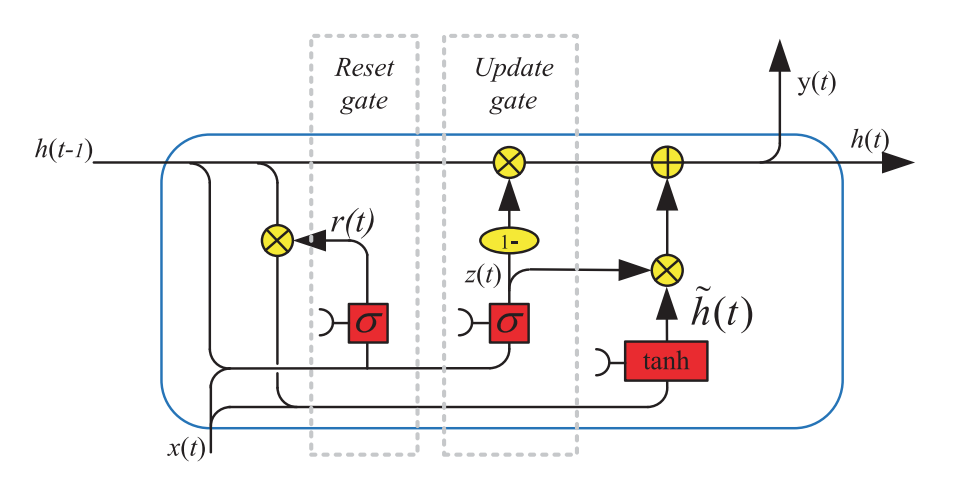
\includegraphics[width=0.8\textwidth]{figures/gru_cell.png}
  \caption{Diagram showing the structure of a GRU cell. This follows the same
    concept as LSTM in that cells have a memory, but now only the input $x(t)$
    is combined with the previous hidden state $h(t-1)$ to form the new output
    $y(t)$ and hidden state $h(t)$. Figure taken
  from~\cite{yu2019review}.}\label{fig:gru_cell}
\end{figure}

The reduction in parameters and number of gates does mean that the GRU is less
powerful than the LSTM and does not work for problems such as
translation~\cite{britz2017massive}. However, it has been applied to birdsong
related problems with promising
results~\cite{parrilla2022polyphonic,adavanne2017stacked}.

While the usage of RNNs, LSTMs or GRUs alone for birdsong classification has
been rare in the literature, there are several examples of experiments where
convolutional layers and recurrent layers have been combined to form a
Convolutional Recurrent Neural Network
(CRNN)~\cite{yan2021birdsong,mukherjee2018convolutional} to leverage
the benefits of both architectures. A typical approach using a CRNN with regards
to birdsong classification might look something like the
following~\cite{crous2019polyphonic}:

\begin{enumerate}

  \item Convert an audio segment to a frequency domain representation to be
    interpreted as an image, e.g.\ a spectrogram. Ideally the image will encode
    some form of temporal evolution to be utilised by the recurrent layers later
    on.

  \item Apply a convolutional layer (or layers) to each time step of the
    representation to extract local features. A time step is defined as
    a single unit along the time axis of the spectrogram.

  \item Apply a recurrent layer to spread the local features of a single time
    step to its temporal surroundings. The spread features can then be processed
    by a fully connected layer with softmax activation as described in
    Section~\ref{ssec:nn} to make a prediction in the form of a distribution
    over output classes for each time step.

\end{enumerate}

The recurrent layer provides two key advantages compared to a plain CNN\@.
Firstly, the network will be able to learn from previous and future features in
order to strengthen predictions. For example, if the current time step equally
supports a blackbird or a nightingale prediction by itself, it will be skewed
towards a blackbird if the previous time step and future time step both
predicted a blackbird. Secondly, the network can learn to include moments of
silence in a prediction. Note that this benefit is lost if just considering
audio segments of isolated syllables as these segments should contain little or
no silence.
